\documentclass[]{nd}
\usepackage[maxcitenames=2,usetranslator=true,hyperref=true,backend=biber,style=nd]{biblatex}
\addbibresource{ref.bib}
\usepackage{graphicx}

\university{Taihoku Imperial University}{臺北帝國大學}
\college{College of Humanity and Political Sciences}{文政學部}
\institute{Graduate Institute of Tridemism}{三民主義研究所}
\degree{Doctoral Dissertation}{博士論文}
\title{Soviet Russia in China: a Summing Up at Seventy}{蘇俄在中國——中國與俄共三十年經歷紀要}
\author{Ishida, Yūsuke}{常凱申}
\advisor{Hsisheng Tao}{陶匯曾\ 先生}
\defenseyear{1956}{45}
\defensemonth{December}{12}

\begin{document}
\makecover
\chapter*{摘要}
摘要\\

\noindent
關鍵字:


\chapter*{Abstract}
Abstract\\

\noindent
Keywords: 
\tableofcontents
\listoffiguresandtables
\mainmatter


\chapter{緒論}
中國 國父孫中山先生,距美國獨立宣言之後一百一十年即在乙酉年(一八八五年),開始宣傳其革命主義。至甲午年(一八九四年),創立其革命總部—興中會於檀香山,成爲中國第一個革命政黨,就揭櫫其推翻中國已有四千年歷史的君主政體的主張。惟其當時的號召,雖爲推翻滿清專制,而其最後的目的則在使中國自列強侵略下獲得解放,並使中國步入政治和社會的民主大道。

\chapter{中俄和平共存的開始}

\section{中俄和平共存的第一個時期}

\section{中國的革命建國運動}

\chapter{測試區}

幾種引用:

\cite{洛克政府論}

\ycite{洛克政府論}

\citeay{洛克政府論}

\citep{洛克政府論}{99}

\pcite{洛克政府論}{99}

\vspace{2cm}

圖片:

\begin{figure}[htp]
    \begin{center}
        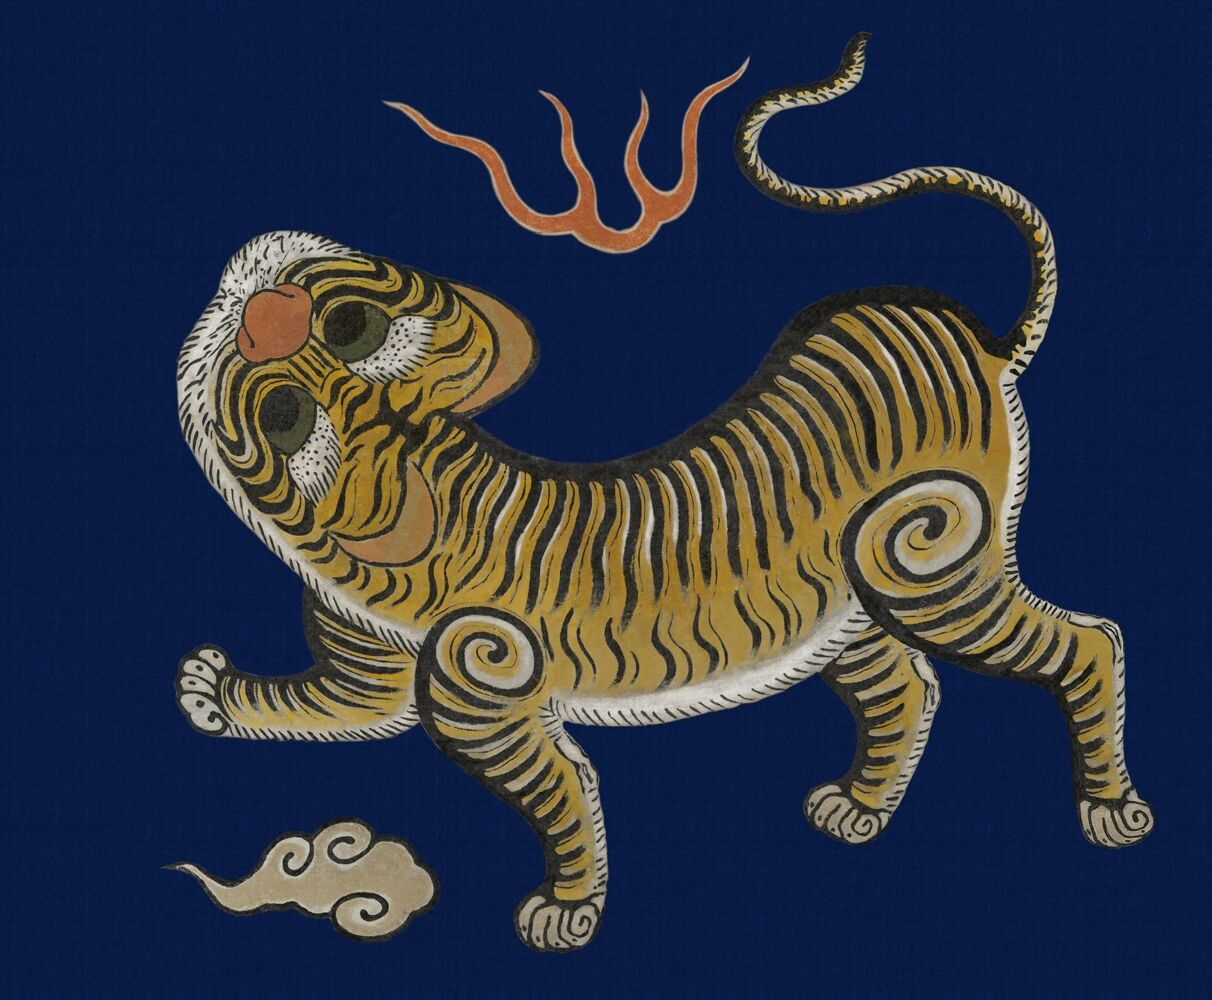
\includegraphics[width=450pt]{tiger.jpeg}
        \caption{臺灣民主國}
        \label{fig:arch_02}
    \end{center}
\end{figure}

表格:

\begin{table}[htbp]
\centering
\begin{tabular}{ccc}
校長 & 任期 & 備註\\
\hline
SCL & 2005.6.22 -- 2013.6.20 & 東方神秘力量研究權威\\
PCY & 2013.6.21 -- 2017.6.21 & 研究誠信辦公室創辦人\\
CRC & 2017.6.22 -- 2017.9.30 & 參選校長失利\\
TWK & 2017.10.1 -- ?? & 代理\\
CMK & 未上任 & 人事聘書未核准\\
\end{tabular}
\caption{臺北帝國大學校長}
\end{table}

\nocite{*}
\printbibliography[heading=bibintoc]

\end{document}